\chapter{Retrieval-Augmented Generation in Recommendation System}
\pagestyle{fancy}\lhead{\textbf \footnotesize\it{Retrieval-Augmented Generation in Recommendation System}}
\pagestyle{fancy}\chead{} \pagestyle{fancy}\rhead{}

 \pagestyle{fancy}\rfoot{\thepage}
%%%%%%%%%%%%%%%%%%%%%%%%%%%%%%%%%%%%%%%%
\section{Introduction}\label{start 1}

LLMs have seen significant advancements but face challenges, particularly in tasks that demand extensive knowledge or deal with queries beyond their training data. These limitations often result in inaccuracies or “hallucinations.” To address this, Retrieval-Augmented Generation (RAG) supplements LLMs by combining information retrieval with text generation to produce more accurate and knowledge-informed outputs. This has led to the widespread adoption of RAG, particularly in chatbots and other real-world applications.

This chapter introduces the concept of RAG, outlines its historical development, It then explores RAG’s core components followed by a classification of its system types. Applications in legal information retrieval are highlighted, alongside evaluation methods and key challenges. The chapter concludes by linking RAG to its role in recommendation systems and domain-specific data processing.

\section{Retrieval-Augmented Generation (RAG)}
RAG represents a significant advancement in the capabilities of LLMs. Understanding the individual components of retrieval and generation is essential to appreciate how their synergy improves the overall performance of RAG systems.
\subsection{Definition of RAG}
Retrieval-Augmented Generation is an advanced neural framework that integrates the generative capabilities of LLMs with external information retrieval mechanisms to improve factual accuracy and contextual relevance ~\citep{selvaraj2024}. Unlike conventional LLMs that rely solely on pre-trained parameters, RAG systems dynamically retrieve relevant documents or from external sources at inference time. 

As formalized by \citep{lewis2020retrieval}, this framework first retrieves relevant documents from a knowledge source, then conditions the language model on this retrieved context to produce more factual and up-to-date outputs. The approach effectively addresses the knowledge limitations of purely parametric models.

IBM Research \citep{ibm2024} describes RAG as a method for augmenting LLMs with retrieval modules, thereby allowing them to access real-time or domain-specific knowledge during generation~.  

Collectively, these perspectives highlight RAG's role in bridging the limitations of static language models by integrating dynamic, context-aware retrieval into the generative process.

\subsection{Historical Development of RAG}
The foundations of RAG can be traced back to traditional information retrieval (IR) systems,  Early models primarily relied on keyword matching and simple ranking mechanisms to retrieve relevant documents from databases, establishing a basic framework for information access. The landscape began to shift with the rise of neural networks in the 2010s\citep{gao2024retrieval}. Notable innovations like Word2Vec and Transformer-based architectures enabled retrieval methods to incorporate deeper semantic understanding, paving the way for more sophisticated document retrieval processes.

A significant advancement occurred with the introduction of dense passage retrieval (DPR) in 2020, which utilized bi-encoder architectures to map both queries and documents into dense vector spaces\citep{gao2024retrieval}. 
The integration of these advanced retrieval techniques with LLMs became a focal point as models like GPT-3 gained prominence. Researchers explored how LLMs could be augmented with retrieval capabilities, leading to the development of RAG systems that leverage the strengths of both retrieval and generative capabilities.
\subsection{Comparison with Fine-Tuning and Transfer Learning}
Recent advances in NLP have led to the development of three prominent methodologies for enhancing language models: RAG, fine-tuning, and transfer learning.
 \begin{enumerate}
  	\item \textbf{RAG}, integrates external retrieval mechanisms with generative models. This approach enables the model to dynamically access and incorporate relevant information from external knowledge bases during the generation process, thereby addressing limitations in its internal memory and providing more accurate responses for knowledge-intensive tasks.
   \item \textbf{Fine-tuning}, detailed by  \citep{howard2018universal}, involves adapting a pre-trained model to a specific task by further training it on a targeted dataset. This process refines the model’s parameters to better capture the nuances of the task at hand, leading to improved performance even when the available domain-specific data is relatively limited.
   \item \textbf{Transfer learning}, as exemplified by \citep{devlin2018bert}, refers to the broader strategy of leveraging a model that has been pre-trained on large, diverse datasets for use in various downstream tasks. This method capitalizes on the rich, generalized representations learned during the pre-training phase, and then applies task-specific adaptations to achieve state-of-the-art results across a range of applications.
	 
\end{enumerate}
Collectively, these methodologies offer complementary strategies to enhance language model performance.

\subsection{Retrieval Mechanism}
RAG systems combine parametric memory (a pre-trained language model) with non-parametric memory (a retrieval mechanism)\citep{zhao2024retrieval}.

The retrieval mechanism allows RAG models to access external information sources (e.g., Wikipedia), and this process is central to improving the model's ability to generate factual and accurate outputs .
\begin{itemize}
	\item\textbf{Traditional Techniques:} 
	Classical retrieval methods include \textbf{TF-IDF and BM25}, which rely on \textbf{sparse vector} representations based on term frequencies. These methods use exact keyword matching, making them limited in semantic understanding.
	\item \textbf{Modern Retrieval Approaches:}
	\textbf{Dense Passage Retrieval (DPR): }This approach utilizes dense vector representations learned by neural models like BERT to encode both the query and document. It allows for a more semantic understanding of the content, making retrieval more effective\citep{karpukhin2020dense}. DPR, for example, computes the similarity between the query and documents using Maximum Inner Product Search (MIPS), which finds the closest passages based on the dense vector space.
	\item \textbf{Others :}
	Beyond conventional sparse and dense retrieval approaches, researchers have developed several specialized techniques for relevance matching. These include:
	\textbf{Structural Similarity Methods}:
	Direct comparison of raw text using edit distance metrics, Syntax-aware matching through \textbf{abstract syntax tree (AST)} comparison for code retrieval.
    These approaches demonstrate the flexibility of retrieval mechanisms in RAG systems, particularly for domain-specific applications where traditional embedding-based methods may be suboptimal.
	
\end{itemize}

\subsection{Generation Process}
The generation in RAG occurs through a combination of retrieved passages and the input query.

Large Language Models LLMs like BART or T5 are utilized for this generation, leveraging their advanced capabilities in understanding and producing human-like text. The retrieval component supplies external context, which the generator conditions on to formulate a response. This context is crucial, as it enriches the LLM's understanding, enabling it to incorporate real-time, relevant information\citep{gupta2024comprehensive}. Moreover, the generation process benefits from the LLM's ability to synthesize information, allowing it to create responses that are not only coherent but also informed by the latest data, thus improving accuracy and relevance in knowledge-intensive tasks  \\
\begin{figure}[h]
	\centering
	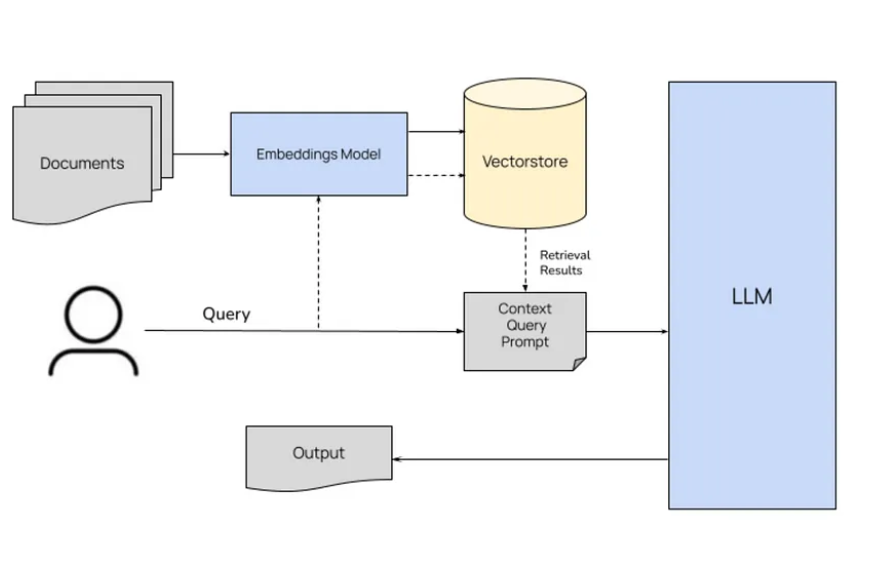
\includegraphics[width=0.9\linewidth]{Figures/rag_architectur.png}
	\caption{Retrieval-Augmented Generation architecture}
	\label{rag_architectur.png}
\end{figure}

\subsection{Augmentation Techniques}
The augmentation of the retrieval process in RAG systems focuses on improving how queries are refined and how relevant information is retrieved for downstream generation tasks. Key augmentation methods include.
\begin{itemize}
	\item \textbf{Query Augmentation:} In traditional retrieval pipelines, user queries are often under-specified or ambiguous, leading to poor retrieval performance. Query augmentation involves dynamically rewriting the user's query to better match the documents in the knowledge base\citep{mombaerts2024meta}. This can be done by leveraging LLMs to generate tailored queries or synthetic questions and answers QAs that better align with the search objective​ .
	\item \textbf{Synthetic QA Generation:} Instead of using raw document chunks, retrieval is enhanced by generating and embedding synthetic QA pairs from documents\citep{mombaerts2024meta}. This helps to capture the semantic essence of long texts more effectively, reducing noise and improving retrieval precision. These synthetic QAs can be used to rewrite the user query, making it more specific to the task at hand .
\end{itemize}

\subsection{Types of RAG Systems}
Recent scholarship has identified four key paradigms in RAG development\citep{gao2024retrieval, ahmed2024agenticrag}.
\begin{figure}[h]
	\centering
	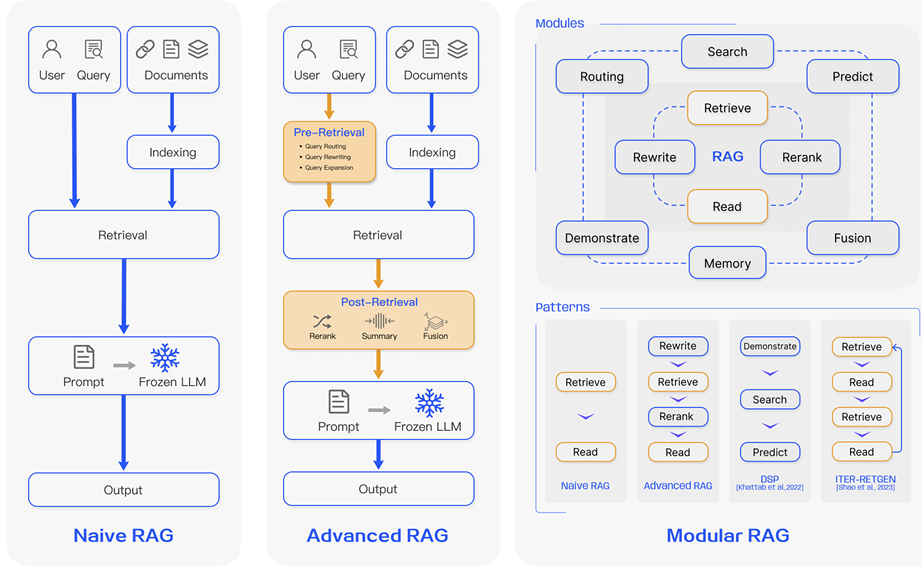
\includegraphics[width=0.9\linewidth]{Figures/rag_types.png}
	\caption{Types of RAG Systems}
	\label{rag_archi}
\end{figure}

\subsection{Naive RAG}
Naive RAG, a foundational approach in RAG, operates on a straightforward "Retrieve-Read-Generate" paradigm. This method involves three primary steps:

\begin{itemize}
	\item \textbf{Indexing:} Raw data is cleaned, extracted, and converted into a uniform text format. It's then segmented into smaller chunks and encoded into vector representations using an embedding model. These vectors are stored in a vector database for efficient similarity searches.
	\item \textbf{Retrieval:} When a user query is received, it's encoded into a vector and compared to the indexed chunks. The top K most similar chunks are retrieved and included in the prompt for the language model.
	\item \textbf{Generation:} The query and retrieved chunks are combined into a prompt, which is fed to a large language model. The model generates a response based on the provided context and its internal knowledge.
\end{itemize}
While Naive RAG offers a basic framework, it faces several challenges in 
\begin{itemize}
	\item\textbf{Retrieval Issues:} The retrieval process can be imprecise, leading to the selection of irrelevant or missing information.
	\item \textbf{Generation Challenges:} The language model may hallucinate, generating content not supported by the retrieved context. It may also produce irrelevant, or biased outputs.
	\item \textbf{Augmentation Difficulties:} Integrating retrieved information into the generation process can be challenging, leading to disjointed or redundant responses.
\end{itemize}

\subsection{Advanced RAG}
Taking aim at the shortcomings of Naive RAG, Advanced RAG introduces specific improvements to enhance retrieval quality. This approach utilizes pre-retrieval and post-retrieval strategies.
\begin{enumerate}
\item \textbf{Pre-retrieval Strategies:}
\begin{itemize}
	\item\textbf{Enhanced Indexing:}Advanced RAG tackles indexing issues through a sliding window approach, finer segmentation of data, and inclusion of metadata. Additionally, it optimizes the retrieval process by employing various methods.
	\item \textbf{Query Optimization:}This stage focuses on refining the user's initial query to make it clearer and more suitable for retrieval. Techniques like query rewriting, transformation are commonly used.
\end{itemize}
\item \textbf{Post-Retrieval Strategies:}
\begin{itemize}
	\item \textbf{Re-ranking Chunks:}After relevant information is retrieved, Advanced RAG prioritizes the most relevant content by re-ranking the retrieved chunks and placing them strategically within the prompt.
	\item \textbf{Context Compression:}To avoid overwhelming the LLM with too much information, post-retrieval efforts focus on selecting the most essential parts of the retrieved context, highlighting critical sections, and compressing the data to be processed.
\end{itemize}
\end{enumerate}
\subsection{Modular RAG} 
Modular RAG represents the latest evolution in RAG, offering greater adaptability. It introduces specialized modules and innovative patterns to enhance retrieval and processing capabilities.
\begin{enumerate}
	
\item \textbf{New Modules}
\begin{itemize}
	\item \textbf{Search Module}: Adapts to specific scenarios by leveraging LLM-generated code and query languages to search across various data sources.
	\item \textbf{RAG Fusion:} Employs a multi-query strategy to expand user queries, uncover both explicit and implicit knowledge, and improve retrieval results.
	\item\textbf{ Memory Module:} Leverages the LLM's memory to guide retrieval and create an unbounded memory pool, aligning the text more closely with data distribution.
	\item \textbf{Routing Module:} Navigates through diverse data sources, selecting the optimal pathway for a query based on its specific needs.
	\item \textbf{Predict Module: } Reduces redundancy and noise by generating relevant context directly through the LLM.
	\item \textbf{Task Adapter Module:} Tailors RAG to various downstream tasks by automating prompt retrieval and creating task-specific retrievers.
\end{itemize}
\item \textbf{New Patterns} 
\begin{itemize}
	\item \textbf{Innovative Retrieval Strategies:} Techniques like Rewrite-Retrieve-Read, Generate-Read, and leverage the LLM's capabilities to refine queries, generate content, and retrieve information from model weights.
	\item \textbf{Hybrid Retrieval:} Combines keyword, semantic, and vector searches to cater to diverse queries, improving retrieval relevance.
	\item \textbf{Dynamic Module Interaction:} Frameworks like Demonstrate-Search-Predict and ITERRETGEN demonstrate the dynamic use of module outputs to enhance each other's functionality.
	\item\textbf{ Adaptive Retrieval:} Techniques like FLARE and Self-RAG evaluate the necessity of retrieval based on different scenarios, allowing for a more flexible and efficient approach.
	
\end{itemize}
\end{enumerate}
\subsection{Agentic RAG}

Agentic Retrieval-Augmented Generation (RAG) enhances conventional RAG frameworks by embedding autonomous, intelligent agents into the pipeline. These agents are designed to dynamically reason, and execute tasks, enabling more flexible and context-aware interactions compared to traditional, static RAG systems. This agent-based approach makes the system significantly more interactive, adaptive, and responsive to diverse user needs\citep{ahmed2024agenticrag}.

Figure\ref{rag_agentic} show architecture of an Agentic RAG system  where an intelligent AI agent orchestrates interactions between the user, external knowledge sources, predefined functions, and a large language model (LLM) to process queries and generate contextually  responses
\begin{figure}[h]
	\centering
	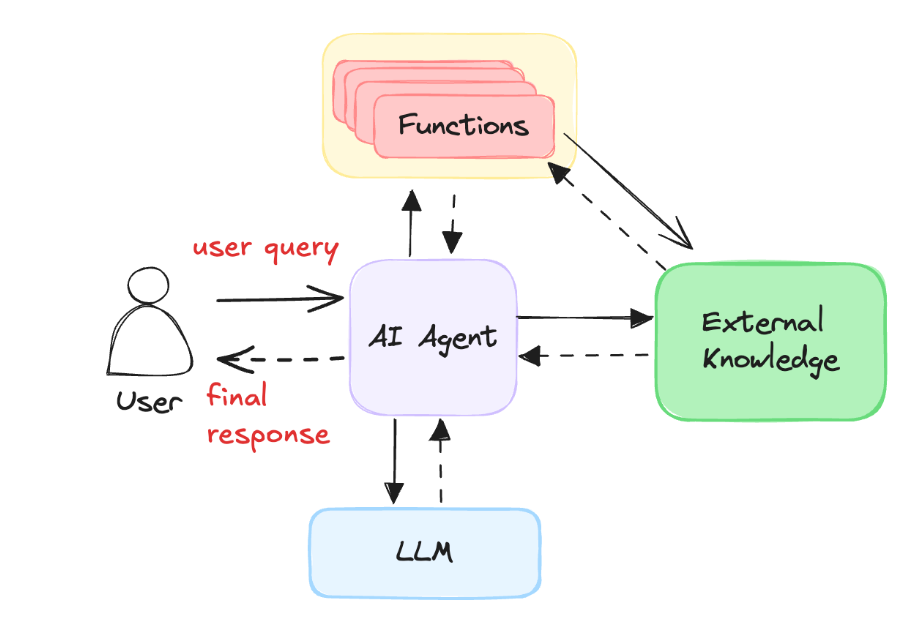
\includegraphics[width=0.7\linewidth]{Figures/agenticrag.png}
\caption{High-level architecture of an Agentic RAG system.}

	\label{rag_agentic}
\end{figure}

Key features of Agentic RAG include:
\begin{itemize}
	\item \textbf{Autonomous Agents:} Responsible for decomposing complex queries, orchestrating the retrieval process, and maintaining relevance in the generated responses.
	\item \textbf{Adaptive Retrieval Pipelines:} Enable real-time modifications to retrieval strategies, allowing the system to better align fetched content with the evolving goals and context of the user.
	\item \textbf{Context-Aware Task Execution:} Agents can coordinate various components (e.g., memory tools, external APIs) to refine their actions based on the specific requirements of each interaction.
	\item \textbf{Improved User Alignment:} Through step-by-step reasoning and continuous feedback loops, agents can better match the user’s intent and deliver more targeted and meaningful outputs.
\end{itemize}


\subsection{Evaluation Methods}
The rapid advancement and widespread adoption of RAG models have made their evaluation a critical area in NLP research~\citep{zhou2020trustworthiness}. The following criteria are commonly used to assess RAG performance:

\begin{enumerate}
	\item \textbf{Factuality:} 
	\begin{itemize}
		\item Use of fact-checking datasets (e.g., FEVER, SQuAD) to assess factual correctness.
		\item Adversarial testing to measure resistance to misleading or incorrect inputs.
		\item Evaluation of contextual understanding for accurate and relevant answers.
	\end{itemize}
	
	\item \textbf{Robustness:}
	\begin{itemize}
		\item Performance under noisy or corrupted retrieval inputs.
		\item Defense against adversarial attacks targeting model reliability.
		\item Adaptability across domains and data shifts.
	\end{itemize}
	
	\item \textbf{Fairness:}
	\begin{itemize}
		\item Detection and quantification of bias in training data and outputs.
		\item Application of fairness metrics such as demographic parity.
		\item Use of mitigation techniques like debiasing and fairness constraints.
	\end{itemize}
	
	\item \textbf{Objective Metrics:}
	\begin{itemize}
		\item Accuracy-related metrics (e.g., precision, recall, F1-score).
		\item Consistency across contexts and queries.
		\item Text coherence and fluency of generated responses.
	\end{itemize}
	
	\item \textbf{Subjective Metrics:}
	\begin{itemize}
		\item Human evaluations to judge quality and usefulness.
		\item User studies for real-world experience and satisfaction.
	\end{itemize}
\end{enumerate}

\subsection{Challenges and Limitations}
While RAG has demonstrated impressive performance across various NLP applications, it is still subject to several technical and practical limitations~\citep{zhao2024retrieval, gupta2024comprehensive}. These challenges span computational efficiency, data quality, fairness, and system complexity:

\begin{enumerate}
	\item \textbf{Scalability and Efficiency:} RAG models often depend on large and continuously growing external corpora, requiring robust and scalable retrieval mechanisms. Managing vast datasets imposes heavy computational and memory demands, which limits the real-time applicability of RAG in resource-constrained settings.
	
	\item \textbf{Noisy Retrieval Results:} The relevance and quality of retrieved documents critically influence the generation quality. Issues such as poorly constructed indices, ambiguous queries, or heterogeneous data sources can lead to noisy or irrelevant results. These, in turn, may trigger hallucinated or inaccurate outputs and hinder the model's capacity to interpret and integrate the retrieved information, especially if inconsistencies or formatting errors exist.
	
	\item \textbf{Bias and Fairness:} RAG systems can inherit and even exacerbate biases present in both the retrieved content and the training data of the generative model. Without effective mitigation strategies, this can lead to biased or unfair outputs, posing risks in sensitive domains like healthcare or law.
	
	\item \textbf{Additional Overhead:}
	\begin{itemize}
		\item \textit{Computational Cost:} RAG introduces extra computational overhead due to the retrieval and integration of external knowledge during inference.
		\item \textit{Latency:} Retrieval steps introduce additional latency, which can hinder user experience in real-time applications.
		\item \textit{System Complexity:} Designing and deploying RAG systems requires coordinating multiple components—retrievers, encoders, decoders—making them more complex to build, maintain, and optimize compared to standalone LLMs.
		
	\end{itemize}
	\item \textbf{Long Context Generation:}
	\begin{itemize}
		\item Context Length Limits: LLMs have limitations on the amount of context they can process at once.
		\item Information Loss: Long documents may be truncated or summarized, leading to loss of important information.
		\item Computational Cost: Processing long contexts can be computationally expensive.
	\end{itemize}
\end{enumerate}

\subsection{State of the Art in Juridical Data}
RAG holds significant promise for transforming the way legal information is accessed, processed, and utilized. In legal contexts, particularly where precision and comprehensiveness are critical, RAG enables the dynamic integration of relevant external knowledge into language models during inference. This is especially valuable for retrieving and synthesizing content from case law, legislative texts, legal commentaries, and scholarly analyses\citep{lexemoRAG}.


\textbf{Evaluating RAG Pipelines for Arabic Lexical Information:} This study, while focused on Arabic lexical retrieval rather than legal texts, offers valuable insights into the performance of various RAG pipelines and Arabic embedding models. 
\citep{arabicrag2024}Explores how well RAG pipelines perform when applied to Arabic lexical information retrieval. The researchers focus on two main components: how different embedding models influence retrieval quality, and how effectively large language models (LLMs) generate relevant and accurate answers in Arabic. They conduct experiments using a dataset of over 88,000 words from the Riyadh Dictionary, evaluating models with metrics like Top-K Recall, MRR, F1 Score, cosine similarity, and accuracy.\\
For embeddings, models like E5-large,  AraBERT, were compared. Results showed that sentence-level embeddings, particularly E5, significantly outperformed word-level ones, with E5 achieving a Top-5 Recall of 88\% and an MRR of 0.48.\\
On the generation side, the team tested models such as GPT-4, GPT-3.5 delivered the best results, reaching an F1 score of 0.90 and an accuracy of 0.82.
\textbf{Hybrid RAG System for Multilingual Legal Information:} 
\citep{legalrag2024} introduces a bilingual QA system tailored for legal documents, specifically the Bangladesh Police Gazettes containing both English and Bangla. The paper presents a hybrid RAG framework that enhances retrieval quality and answer precision. By comparing the proposed model with standard RAG pipelines, the authors  demonstrate significant improvements in retrieving and generating responses to legal queries. This work highlights the potential of advanced NLP techniques in making multilingual regulatory information more accessible and searchable.

\textbf{Multitask Benchmark for Assessing Arabic Legal Knowledge:}
\citep{arablegaleval2024} Introduces a multitask benchmark designed to evaluate the Arabic legal reasoning abilities of large language models (LLMs), a domain that has remained largely underexplored. Inspired by datasets like MMLU and LegalBench, ArabLegalEval includes tasks drawn from Saudi legal texts and automatically validated synthetic questions. The study benchmarks top-performing multilingual and Arabic-focused LLMs (e.g., GPT-4 and Jais), assesses the role of in-context learning, and proposes a robust method for dataset creation and validation that can be adapted to other domains. The authors aim to foster progress in Arabic legal NLP by releasing both the dataset and accompanying tools.

\section{Recommendation Systems}
Modern technology and online services have enabled unprecedented access to vast amounts of data. However, this abundance of information creates an overload, making it harder for users to find relevant content efficiently. Recommender systems address this by filtering information and delivering personalized suggestions.
\subsection{Definition of Recommendation Systems}

A recommendation system is a subclass of information filtering systems that seek to predict the preference a user would give to an item. By analyzing patterns in user behavior and item attributes, these systems aim to present users with items that are most likely to be of interest, thereby enhancing user experience and engagement~\citep{Roy2022}.These systems are now integral to platforms like e-commerce, television programs, e-learning, tourism, and more, though further improvements are needed to enhance their versatility and accuracy.
\begin{figure}[ht]
		\centering
	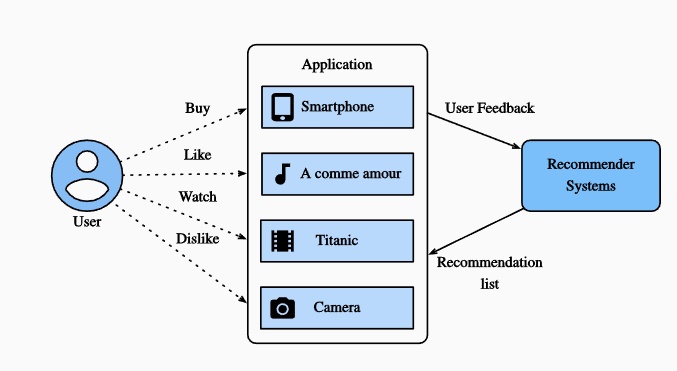
\includegraphics[width=0.7\linewidth]{Figures/RS.png}
	\caption{Recommendation System Process}
	\label{Recommendation_System _Process}	
	\end{figure}

\subsection{Types of Recommendation Systems}

Recommendation systems can be broadly categorized into several types based on their underlying methodologies~\citep{maruti_recsys}:

\begin{enumerate}
	\item \textbf{Content-Based Filtering:} This approach recommends items similar to those the user has liked in the past, based on item features. It relies on the assumption that if a user liked an item, they will also like similar items.
	
	\item \textbf{Collaborative Filtering:} This method predicts user preferences based on the preferences of other users. It operates under the premise that users who agreed in the past will agree in the future about item preferences.
	
	\item \textbf{Hybrid Methods:} These systems  integrate both content-based and collaborative filtering approaches to enhance the accuracy and diversity of suggestions. A well-known example is Netflix, which combines user behavior patterns (e.g., viewing and search history) with similarities across users to implement collaborative filtering, while also recommending content with attributes similar to previously liked items via content-based filtering.
	
	\item \textbf{Sequential Recommendation Models:} These models consider the sequence of user interactions over time to predict future preferences. An example is the Self-Attentive Sequential Recommendation \textbf{(SASRec)} model, which utilizes self-attention mechanisms to capture user behavior patterns effectively. SASRec has demonstrated superior performance in modeling user-item interactions by focusing on the most relevant past actions.
\end{enumerate}

\subsection{Evaluation Metrics}

Evaluating the performance of recommendation systems is crucial for understanding their effectiveness and guiding improvements. Common evaluation metrics include:

\begin{itemize}
	\item \textbf{Hit Rate at \( k \) (HR@\( k \))}: Measures the proportion of cases where the target item appears in the top-\( k \) recommendations. The HR@\( k \) is computed as:\citep{Tamm_2021}
	\begin{equation}
		\text{HR@}k = \frac{1}{|U|} \sum_{u=1}^{|U|} \mathbb{I}(\text{rank}_u \leq k),
	\end{equation}
	where \( |U| \) is the number of users, \( \text{rank}_u \) is the rank of the target item for user \( u \), and \( \mathbb{I}(\cdot) \) is the indicator function that returns 1 if the condition is true and 0 otherwise.
	
	\item \textbf{Mean Reciprocal Rank (MRR)}:is a ranking quality metric that measures how quickly a system retrieves the first relevant item. It is calculated as the average of reciprocal ranks across all users or queries,MRR ranges from 0 to 1, with higher values indicating better performance \citep{Tamm_2021}.
	\begin{equation}
		\text{MRR} = \frac{1}{|U|} \sum_{u=1}^{|U|} \frac{1}{\text{rank}_u},
	\end{equation}
	where \( \text{rank}_u \) is the position of the first relevant item for user \( u \) within the top-K results. \\ 
	U represents the total number of users (for recommendation systems) or queries (for information retrieval tasks) in the dataset.
	
	\item \textbf{Normalized Discounted Cumulative Gain (NDCG)}: Assesses the ranking quality while accounting for position importance. The NDCG@\( k \) is computed as:\citep{Tamm_2021}
	\begin{equation}
		\text{NDCG@}k = \frac{1}{|U|} \sum_{u=1}^{|U|} \frac{\text{DCG@}k}{\text{IDCG@}k},
	\end{equation}
	where \( \text{DCG@}k \) is the Discounted Cumulative Gain at position \( k \):
	\begin{equation}
		\text{DCG@}k = \sum_{i=1}^{k} \frac{2^{\text{rel}_i} - 1}{\log_2(i + 1)},
	\end{equation}
	and \( \text{IDCG@}k \) is the Ideal DCG@\( k \), computed by sorting the items by their true relevance scores.
\end{itemize} 

\subsection{Retrieval-Augmented Generation in Recommendation Systems}

Retrieval-Augmented Generation represents a significant advancement in recommender systems by integrating large language models LLMs with traditional retrieval techniques. This approach enhances recommendation quality by allowing the system to access and incorporate external information into its responses, resulting in more accurate and context-aware suggestions.

In this setup, a RAG-based recommender retrieves relevant data from external sources and feeds it into the language model, which then generates personalized recommendations based on both the retrieved content and user input\citep{DiPalma}. This hybrid mechanism helps overcome common challenges like the cold start problem and data sparsity, enabling effective recommendations even with limited user history.

Recent studies highlight that combining retrieval with LLMs greatly improves the system’s ability to deliver more relevant and diverse content, offering a promising direction for improving user experience in applications such as e-commerce and digital streaming platforms.



\section{Conclusion}


In this chapter, we explored the core principles and mechanisms of RAG, emphasizing its potential to enhance language models through access to external knowledge sources during inference. We examined its general architecture, key stages, and its evolution from naive to more modular frameworks. 

Particular attention was given to RAG’s application in the legal domain, highlighting its ability to enhance legal information retrieval by enabling more contextualized and semantically rich access to case law, statutes, and scholarly texts. We also outlined the main challenges and limitations facing RAG models. Additionally, the chapter briefly touched on the integration of RAG in recommendation systems, introducing its potential to improve personalization and relevance in such applications.

the next chapter addresses a critical factor in RAG performance: knowledge selection. Specifically, we explore how the effectiveness of retrieved documents directly influences the quality of generated responses, and we investigate strategies to improve relevance and ranking within RAG pipelines.
